\chapter{Lukuteoria}

\index{lukuteoria@lukuteoria}

\key{Lukuteoria} on kokonaislukuja tutkiva
matematiikan ala, jonka keskeinen
käsite on lukujen jaollisuus.
Lukuteoriassa on kiehtovaa, että monet kokonaislukuihin
liittyvät kysymykset ovat hyvin vaikeita ratkaista,
vaikka ne saattavat näyttää päältä päin yksinkertaisilta.

Tarkastellaan esimerkkinä seuraavaa yhtälöä:
\[x^3 + y^3 + z^3 = 33\]
On helppoa löytää kolme reaalilukua $x$, $y$ ja $z$,
jotka toteuttavat yhtälön. Voimme valita
esimerkiksi
\[
\begin{array}{lcl}
x = 0, \\
y = 0, \\
z = \sqrt[3]{33}.\\
\end{array}
\]
Sen sijaan kukaan ei tiedä, onko olemassa
kolmea kokonaislukua $x$, $y$ ja $z$,
jotka toteuttaisivat yhtälön, vaan kyseessä
on avoin ongelma.

Tässä luvussa tutustumme lukuteorian peruskäsitteisiin ja
-algoritmeihin.
Lähdemme liikkeelle lukujen jaollisuudesta,
johon liittyvät keskeiset algoritmit ovat
alkuluvun tarkastaminen sekä luvun jakaminen tekijöihin.

\section{Alkuluvut ja tekijät}

\index{jaollisuus@jaollisuus}
\index{jakaja@jakaja}
\index{tekijx@tekijä}

Luku $a$ on luvun $b$ \key{jakaja} eli \key{tekijä},
jos $b$ on jaollinen $a$:lla.
Jos $a$ on $b$:n jakaja,
niin merkitään $a \mid b$,
ja muuten merkitään $a \nmid b$.
Esimerkiksi luvun 24 jakajat ovat 1, 2, 3, 4, 6, 8, 12 ja 24.

\index{alkuluku@alkuluku}
\index{alkutekijxhajotelma@alkutekijähajotelma}

Luku $n$ on \key{alkuluku}, jos sen ainoat 
positiiviset jakajat ovat 1 ja $n$.
Esimerkiksi luvut 7, 19 ja 41 ovat alkulukuja.
Luku 35 taas ei ole alkuluku, koska se voidaan
jakaa tekijöihin $5 \cdot 7 = 35$.
Jokaiselle luvulle $n>1$ on olemassa yksikäsitteinen
\key{alkutekijähajotelma}
\[ n = p_1^{\alpha_1} p_2^{\alpha_2} \cdots p_k^{\alpha_k},\]
missä $p_1,p_2,\ldots,p_k$ ovat alkulukuja
ja $\alpha_1,\alpha_2,\ldots,\alpha_k$ ovat positiivisia
lukuja. Esimerkiksi luvun 84 alkutekijähajotelma on
\[84 = 2^2 \cdot 3^1 \cdot 7^1.\]

Luvun $n$ \key{jakajien määrä} on
\[\tau(n)=\prod_{i=1}^k (\alpha_i+1),\]
koska alkutekijän $p_i$ kohdalla on $\alpha_i+1$
tapaa valita, montako kertaa alkutekijä
esiintyy jakajassa.
Esimerkiksi luvun 84 jakajien määrä
on $\tau(84)=3 \cdot 2 \cdot 2 = 12$.
Jakajat ovat
1, 2, 3, 4, 6, 7, 12, 14, 21, 28, 42 ja 84.

Luvun $n$ \key{jakajien summa} on
\[\sigma(n)=\prod_{i=1}^k (1+p_1+\ldots+p_1^{\alpha_i}) = \prod_{i=1}^k \frac{p_i^{a_i+1}-1}{p_i-1},\]
missä jälkimmäinen muoto perustuu geometriseen summaan.
Esimerkiksi luvun 84 jakajien summa on
\[\sigma(84)=\frac{2^3-1}{2-1} \cdot \frac{3^2-1}{3-1} \cdot \frac{7^2-1}{7-1} = 7 \cdot 4 \cdot 8 = 224.\]

Luvun $n$ \key{jakajien tulo} on
\[\mu(n)=n^{\tau(n)/2},\]
koska jakajista voi muodostaa
$\tau(n)/2$ paria, joiden jokaisen tulona on $n$.
Esimerkiksi luvun 84 jakajista muodostuu parit
$1 \cdot 84$, $2 \cdot 42$, $3 \cdot 28$, jne.,
ja jakajien tulo on $\pi(84)=84^6=351298031616$.

%\index{tzydellinen luku@täydellinen luku}
\index{txydellinen luku@täydellinen luku}

Luku $n$ on \key{täydellinen}, jos $n=\sigma(n)-n$
eli luku on yhtä suuri kuin summa sen jakajista
välillä $1 \ldots n-1$.
Esimerkiksi luku 28 on täydellinen, koska
se muodostuu summana $1+2+4+7+14$.

\subsubsection{Alkulukujen määrä}

On helppoa osoittaa, että alkulukuja on äärettömästi.
Jos nimittäin alkulukuja olisi äärellinen määrä,
voisimme muodostaa joukon $P=\{p_1,p_2,\ldots,p_n\}$,
joka sisältää kaikki alkuluvut.
Esimerkiksi $p_1=2$, $p_2=3$, $p_3=5$, jne.

Nyt kuitenkin voisimme muodostaa uuden alkuluvun
\[p_1 p_2 \cdots p_n+1,\]
joka on kaikkia $P$:n lukuja suurempi.
Koska tätä lukua ei ole joukossa $P$,
syntyy ristiriita ja alkulukujen määrän on
pakko olla ääretön.

\subsubsection{Alkulukujen tiheys}

Alkulukujen tiheys tarkoittaa, kuinka usein alkulukuja
esiintyy muiden lukujen joukossa.
Merkitään funktiolla $\pi(n)$, 
montako alkulukua on välillä $1 \ldots n$.
Esimerkiksi $\pi(10)=4$, koska välillä $1 \ldots 10$
on alkuluvut 2, 3, 5 ja 7.

On mahdollista osoittaa, että
\[\pi(n) \approx \frac{n}{\ln n},\]
mikä tarkoittaa, että alkulukuja esiintyy
varsin usein. Esimerkiksi alkulukujen määrä
välillä $1 \ldots 10^6$ on $\pi(10^6)=78498$
ja $10^6 / \ln 10^6 \approx 72382$.

\subsubsection{Konjektuureja}

Alkulukuihin liittyy useita konjektuureja
eli lauseita, joiden uskotaan olevan tosia mutta
joita kukaan ei ole onnistunut todistamaan tähän mennessä.
Kuuluisia konjektuureja ovat seuraavat:

\begin{itemize}
\index{Goldbachin konjektuuri@Goldbachin konjektuuri}
\item \key{Goldbachin konjektuuri}:
Jokainen parillinen kokonaisluku $n>2$ voidaan esittää
muodossa $n=a+b$ niin, että $a$ ja $b$
ovat alkulukuja.
\index{alkulukupari@alkulukupari}
\item \key{Alkulukuparit}:
On olemassa äärettömästi pareja muotoa $\{p,p+2\}$,
joissa sekä $p$ että $p+2$ on alkuluku.
\index{Legendren konjektuuri@Legendren konjektuuri}
\item \key{Legendren konjektuuri}:
Lukujen $n^2$ ja $(n+1)^2$ välillä on aina alkuluku,
kun $n$ on mikä tahansa positiivinen kokonaisluku.
\end{itemize}

\subsubsection{Perusalgoritmit}

Jos luku $n$ ei ole alkuluku,
niin sen voi esittää muodossa $a \cdot b$,
missä $a \le \sqrt n$ tai $b \le \sqrt n$,
minkä ansiosta sillä on varmasti
tekijä välillä $2 \ldots \sqrt n$.
Tämän havainnon avulla voi tarkastaa ajassa $O(\sqrt n)$,
onko luku alkuluku,
sekä myös selvittää ajassa $O(\sqrt n)$
luvun alkutekijät.

Seuraava funktio \texttt{alkuluku} tutkii,
onko annettu luku $n$ alkuluku.
Funktio koettaa jakaa lukua kaikilla luvuilla
välillä $2 \ldots \sqrt n$, ja jos mikään
luvuista ei jaa $n$:ää, niin $n$ on alkuluku.

\begin{lstlisting}
bool alkuluku(int n) {
    if (n < 2) return false;
    for (int x = 2; x*x <= n; x++) {
        if (n%x == 0) return false;
    }
    return true;
}
\end{lstlisting}

\noindent
Seuraava funktio \texttt{tekijat} muodostaa
vektorin, joka sisältää luvun $n$
alkutekijät.
Funktio jakaa $n$:ää sen alkutekijöillä ja lisää
niitä samaan aikaan vektoriin.
Prosessi päättyy, kun jäljellä on luku $n$,
jolla ei ole tekijää välillä $2 \ldots \sqrt n$.
Jos $n>1$, se on alkuluku ja viimeinen tekijä.

\begin{lstlisting}
vector<int> tekijat(int n) {
    vector<int> f;
    for (int x = 2; x*x <= n; x++) {
        while (n%x == 0) {
            f.push_back(x);
            n /= x;
        }
    }
    if (n > 1) f.push_back(n);
    return f;
}
\end{lstlisting}

Huomaa, että funktio lisää jokaisen
alkutekijän vektoriin
niin monta kertaa, kuin kyseinen
alkutekijä jakaa luvun.
Esimerkiksi $24=2^3 \cdot 3$,
joten funktio muodostaa vektorin $[2,2,2,3]$.

\subsubsection{Eratostheneen seula}

\index{Eratostheneen seula@Eratostheneen seula}

\key{Eratostheneen seula} on esilaskenta-algoritmi,
jonka suorituksen jälkeen mistä tahansa
välin $2 \ldots n$ luvusta pystyy tarkastamaan
nopeasti, onko se alkuluku,
sekä etsimään yhden luvun alkutekijän,
jos luku ei ole alkuluku.

Algoritmi luo taulukon $\texttt{a}$,
jossa on käytössä indeksit $2,3,\ldots,n$.
Taulukossa $\texttt{a}[k]=0$ tarkoittaa,
että $k$ on alkuluku,
ja $\texttt{a}[k] \neq 0$ tarkoittaa,
että $k$ ei ole alkuluku.
Jälkimmäisessä tapauksessa $\texttt{a}[k]$
on yksi $k$:n alkutekijöistä.

Algoritmi käy läpi välin
$2 \ldots n$ luvut yksi kerrallaan.
Aina kun vastaan tulee uusi alkuluku $x$,
niin algoritmi merkitsee taulukkoon, että $x$:n moninkerrat
$2x,3x,4x,\ldots$ eivät ole alkulukuja,
koska niillä on alkutekijä $x$.

Esimerkiksi jos $n=20$,
taulukosta tulee:

\begin{center}
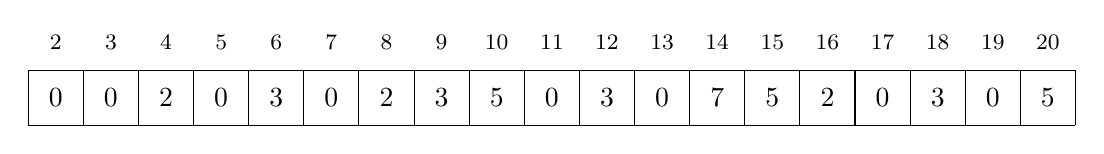
\begin{tikzpicture}[scale=0.7]
\draw (0,0) grid (19,1);

\node at (0.5,0.5) {$0$};
\node at (1.5,0.5) {$0$};
\node at (2.5,0.5) {$2$};
\node at (3.5,0.5) {$0$};
\node at (4.5,0.5) {$3$};
\node at (5.5,0.5) {$0$};
\node at (6.5,0.5) {$2$};
\node at (7.5,0.5) {$3$};
\node at (8.5,0.5) {$5$};
\node at (9.5,0.5) {$0$};
\node at (10.5,0.5) {$3$};
\node at (11.5,0.5) {$0$};
\node at (12.5,0.5) {$7$};
\node at (13.5,0.5) {$5$};
\node at (14.5,0.5) {$2$};
\node at (15.5,0.5) {$0$};
\node at (16.5,0.5) {$3$};
\node at (17.5,0.5) {$0$};
\node at (18.5,0.5) {$5$};

\footnotesize

\node at (0.5,1.5) {$2$};
\node at (1.5,1.5) {$3$};
\node at (2.5,1.5) {$4$};
\node at (3.5,1.5) {$5$};
\node at (4.5,1.5) {$6$};
\node at (5.5,1.5) {$7$};
\node at (6.5,1.5) {$8$};
\node at (7.5,1.5) {$9$};
\node at (8.5,1.5) {$10$};
\node at (9.5,1.5) {$11$};
\node at (10.5,1.5) {$12$};
\node at (11.5,1.5) {$13$};
\node at (12.5,1.5) {$14$};
\node at (13.5,1.5) {$15$};
\node at (14.5,1.5) {$16$};
\node at (15.5,1.5) {$17$};
\node at (16.5,1.5) {$18$};
\node at (17.5,1.5) {$19$};
\node at (18.5,1.5) {$20$};

\end{tikzpicture}
\end{center}

Seuraava koodi muodostaa
Eratostheneen seulan.
Koodi olettaa, että jokainen taulukon \texttt{a}
alkio on aluksi 0.

\begin{lstlisting}
for (int x = 2; x <= n; x++) {
    if (a[x]) continue;
    for (int u = 2*x; u <= n; u += x) {
        a[u] = x;
    }
}
\end{lstlisting}

Algoritmin sisäsilmukka suoritetaan
$n/x$ kertaa tietyllä $x$:n arvolla,
joten yläraja algoritmin ajankäytölle
on harmoninen summa

\index{harmoninen summa@harmoninen summa}

\[\sum_{x=2}^n n/x = n/2 + n/3 + n/4 + \cdots + n/n = O(n \log n).\]

Todellisuudessa algoritmi on vielä nopeampi,
koska sisäsilmukka suoritetaan vain,
jos luku $x$ on alkuluku.
Voidaan osoittaa, että algoritmin aikavaativuus
on vain $O(n \log \log n)$ eli hyvin lähellä $O(n)$.

\subsubsection{Eukleideen algoritmi}

\index{suurin yhteinen tekijx@suurin yhteinen tekijä}
\index{pienin yhteinen moninkerta@pienin yhteinen moninkerta}
\index{Eukleideen algoritmi@Eukleideen algoritmi}

Lukujen $a$ ja $b$ \key{suurin yhteinen tekijä} eli $\textrm{syt}(a,b)$
on suurin luku, jolla sekä $a$ että $b$ on jaollinen.
Lukujen $a$ ja $b$ \key{pienin yhteinen moninkerta} eli $\textrm{pym}(a,b)$
on puolestaan pienin luku, joka on jaollinen sekä $a$:lla että $b$:llä.
Esimerkiksi $\textrm{syt}(24,36)=12$ ja
$\textrm{pym}(24,36)=72$.

Suurimman yhteisen tekijän ja pienimmän yhteisen
moninkerran välillä on yhteys
\[\textrm{pym}(a,b)=\frac{ab}{\textrm{syt}(a,b)}.\]
\key{Eukleideen algoritmi} on tehokas tapa etsiä
suurin yhteinen tekijä.
Se laskee suurimman yhteisen tekijän kaavalla
\begin{equation*}
    \textrm{syt}(a,b) = \begin{cases}
               a        & b = 0\\
               \textrm{syt}(b,a \bmod b) & b \neq 0\\
           \end{cases}
\end{equation*}

\noindent
Esimerkiksi
\[\textrm{syt}(24,36) = \textrm{syt}(36,24)
= \textrm{syt}(24,12) = \textrm{syt}(12,0)=12.\]
Eukleideen algoritmin aikavaativuus
on $O(\log n)$, kun $n=\min(a,b)$.
Pahin tapaus algoritmille on, jos luvut ovat
peräkkäiset Fibonaccin luvut.
Silloin algoritmi käy läpi kaikki pienemmät
peräkkäiset Fibonaccin luvut.
Esimerkiksi
\[\textrm{syt}(13,8)=\textrm{syt}(8,5)
=\textrm{syt}(5,3)=\textrm{syt}(3,2)=\textrm{syt}(2,1)=\textrm{syt}(1,0)=1.\]

\subsubsection{Eulerin totienttifunktio}

\index{suhteellinen alkuluku@suhteellinen alkuluku}
\index{Eulerin totienttifunktio@Eulerin totienttifunktio}

Luvut $a$ ja $b$ ovat suhteelliset alkuluvut,
jos $\textrm{syt}(a,b)=1$.
\key{Eulerin totienttifunktio} $\varphi(n)$
laskee luvun $n$ suhteellisten alkulukujen
määrän välillä $1 \ldots n$.
Esimerkiksi $\varphi(12)=4$,
koska luvut 1, 5, 7 ja 11 ovat suhteellisia
alkulukuja luvun 12:n kanssa.

Totienttifunktion arvon $\varphi(n)$ pystyy laskemaan
luvun $n$ alkutekijähajotelmasta kaavalla
\[ \varphi(n) = \prod_{i=1}^k p_i^{\alpha_i-1}(p_i-1). \]
Esimerkiksi $\varphi(12)=2^1 \cdot (2-1) \cdot 3^0 \cdot (3-1)=4$.
Huomaa myös, että $\varphi(n)=n-1$,
jos $n$ on alkuluku.

\section{Modulolaskenta}

\index{modulolaskenta@modulolaskenta}

\key{Modulolaskennassa} lukualuetta rajoitetaan
niin, että käytössä ovat vain
kokonaisluvut $0,1,2,\ldots,m-1$,
missä $m$ on vakio.
Ideana on, että lukua $x$ kuvaa luku $x \bmod m$
eli luvun $x$ jakojäännös luvulla $m$.
Esimerkiksi jos $m=17$, niin lukua $75$ kuvaa luku
$75 \bmod 17 = 7$.

Useissa laskutoimituksissa jakojäännöksen voi laskea
ennen laskutoimitusta, minkä ansiosta saadaan seuraavat kaavat:
\[
\begin{array}{rcl}
(x+y) \bmod m & = & (x \bmod m + y \bmod m) \bmod m \\
(x-y) \bmod m & = & (x \bmod m - y \bmod m) \bmod m \\
(x \cdot y) \bmod m & = & (x \bmod m \cdot y \bmod m) \bmod m \\
(x^k) \bmod m & = & (x \bmod m)^k \bmod m \\
\end{array}
\]

\subsubsection{Tehokas potenssilasku}

Modulolaskennassa tulee usein tarvetta laskea
tehokkaasti potenssilasku $x^n$.
Tämä onnistuu ajassa $O(\log n)$
seuraavan rekursion avulla:
\begin{equation*}
    x^n = \begin{cases}
               1        & n = 0\\
               x^{n/2} \cdot x^{n/2} & \text{$n$ on parillinen}\\
               x^{n-1} \cdot x & \text{$n$ on pariton}
           \end{cases}
\end{equation*}

Oleellista on, että parillisen $n$:n
tapauksessa luku $x^{n/2}$ lasketaan vain kerran.
Tämän ansiosta potenssilaskun aikavaativuus on $O(\log n)$,
koska $n$:n koko puolittuu aina silloin,
kun $n$ on parillinen.

Seuraava funktio laskee luvun $x^n \bmod m$:

\begin{lstlisting}
int pot(int x, int n, int m) {
    if (n == 0) return 1%m;
    int u = pot(x,n/2,m);
    u = (u*u)%m;
    if (n%2 == 1) u = (u*x)%m;
    return u;
}
\end{lstlisting}

\subsubsection{Fermat'n pieni lause ja Eulerin lause}

\index{Fermat'n pieni lause}
\index{Eulerin lause@Eulerin lause}

\key{Fermat'n pienen lauseen} mukaan
\[x^{m-1} \bmod m = 1,\]
kun $m$ on alkuluku ja $x$ ja $m$ ovat suhteelliset alkuluvut.
Tällöin myös
\[x^k \bmod m = (x^{k \bmod (m-1)}) \bmod m.\]
Yleisemmin \key{Eulerin lauseen} mukaan
\[x^{\varphi(m)} \bmod m = 1,\]
kun $x$ ja $m$ ovat suhteelliset alkuluvut.
Fermat'n pieni lause seuraa Eulerin lauseesta,
koska jos $m$ on alkuluku, niin $\varphi(m)=m-1$.

\subsubsection{Modulon käänteisluku}

\index{modulon kxxnteisluku@modulon käänteisluku}

Luvun $x$ käänteisluku modulo $m$
tarkoittaa sellaista lukua $x^{-1}$,
että
\[ x x^{-1} \bmod m = 1. \]
Esimerkiksi jos $x=6$ ja $m=17$,
niin $x^{-1}=3$, koska $6\cdot3 \bmod 17=1$.

Modulon käänteisluku mahdollistaa
jakolaskun laskemisen modulossa,
koska jakolasku luvulla $x$ vastaa
kertolaskua luvulla $x^{-1}$.
Esimerkiksi jos haluamme laskea
jakolaskun $36/6 \bmod 17$,
voimme muuttaa sen muotoon  $2 \cdot 3 \bmod 17$,
koska $36 \bmod 17 = 2$ ja $6^{-1} \bmod 17 = 3$.

Modulon käänteislukua ei
kuitenkaan ole aina olemassa.
Esimerkiksi jos $x=2$ ja $m=4$,
yhtälölle
\[ x x^{-1} \bmod m = 1. \]
ei ole ratkaisua, koska kaikki luvun 2
moninkerrat ovat parillisia eikä jakojäännös
4:llä voi koskaan olla 1.
Osoittautuu, että $x^{-1} \bmod m$
on olemassa tarkalleen silloin,
kun $x$ ja $m$ ovat suhteelliset alkuluvut.

Jos modulon käänteisluku on olemassa,
sen saa laskettua kaavalla
\[
x^{-1} = x^{\varphi(m)-1}.
\]
Erityisesti jos $m$ on alkuluku, kaavasta tulee
\[
x^{-1} = x^{m-2}.
\]
Esimerkiksi jos $x=6$ ja $m=17$, niin
\[x^{-1}=6^{17-2} \bmod 17 = 3.\]
Tämän kaavan ansiosta modulon käänteisluvun pystyy
laskemaan nopeasti tehokkaan potenssilaskun avulla.

Modulon käänteisluvun kaavan voi perustella Eulerin lauseen avulla.
Ensinnäkin käänteisluvulle täytyy päteä
\[
x x^{-1} \bmod m = 1.
\]
Toisaalta Eulerin lauseen mukaan
\[
x^{\varphi(m)} \bmod m =  xx^{\varphi(m)-1} \bmod m = 1,
\]
joten lukujen $x^{-1}$ ja $x^{\varphi(m)-1}$ on oltava samat.

\subsubsection{Modulot tietokoneessa}

Tietokone käsittelee etumerkittömiä kokonaislukuja
modulo $2^k$, missä $k$ on luvun bittien määrä.
Usein näkyvä seuraus tästä on luvun arvon pyörähtäminen
ympäri, jos luku kasvaa liian suureksi.

Esimerkiksi C++:ssa \texttt{unsigned int} -tyyppinen
arvo lasketaan modulo $2^{32}$.
Seuraava koodi määrittelee muuttujan
tyyppiä \texttt{unsigned int},
joka saa arvon $123456789$.
Sitten muuttujan arvo kerrotaan itsellään,
jolloin tuloksena on luku 
$123456789^2 \bmod 2^{32} = 2537071545$.

\begin{lstlisting}
unsigned int x = 123456789;
cout << x*x << "\n"; // 2537071545
\end{lstlisting}

\section{Yhtälönratkaisu}

\index{Diofantoksen yhtxlz@Diofantoksen yhtälö}

\key{Diofantoksen yhtälö} on muotoa
\[ ax + by = c, \]
missä $a$, $b$ ja $c$ ovat vakioita
ja tehtävänä on ratkaista muuttujat $x$ ja $y$.
Jokaisen yhtälössä esiintyvän luvun tulee
olla kokonaisluku.
Esimerkiksi jos yhtälö on $5x+2y=11$, yksi ratkaisu
on valita $x=3$ ja $y=-2$.

\index{Eukleideen algoritmi@Eukleideen algoritmi}

Diofantoksen yhtälön voi ratkaista
tehokkaasti Eukleideen algoritmin avulla,
koska Eukleideen algoritmia laajentamalla
pystyy löytämään luvun $\textrm{syt}(a,b)$
lisäksi luvut $x$ ja $y$,
jotka toteuttavat yhtälön
\[
ax + by = \textrm{syt}(a,b).
\]

Diofantoksen yhtälön ratkaisu on olemassa, jos $c$ on
jaollinen $\textrm{syt}(a,b)$:llä,
ja muussa tapauksessa yhtälöllä ei ole ratkaisua.

\index{laajennettu Eukleideen algoritmi@laajennettu Eukleideen algoritmi}

\subsubsection*{Laajennettu Eukleideen algoritmi}

Etsitään esimerkkinä luvut $x$ ja $y$,
jotka toteuttavat yhtälön
\[
39x + 15y = 12.
\]
Yhtälöllä on ratkaisu, koska $\textrm{syt}(39,15)=3$
ja $3 \mid 12$.
Kun Eukleideen algoritmi laskee lukujen
39 ja 15 suurimman
yhteisen tekijän, syntyy ketju
\[
\textrm{syt}(39,15) = \textrm{syt}(15,9)
= \textrm{syt}(9,6) = \textrm{syt}(6,3)
= \textrm{syt}(3,0) = 3. \]
Algoritmin aikana muodostuvat jakoyhtälöt ovat:
\[
\begin{array}{lcl}
39 - 2 \cdot 15 & = & 9 \\
15 - 1 \cdot 9 & = & 6 \\
9 - 1 \cdot 6 & = & 3 \\
\end{array}
\]
Näiden yhtälöiden avulla saadaan
\[
39 \cdot 2 + 15 \cdot (-5) = 3
\]
ja kertomalla yhtälö 4:lla tuloksena on
\[
39 \cdot 8 + 15 \cdot (-20) = 12,
\]
joten alkuperäisen yhtälön ratkaisu on $x=8$ ja $y=-20$.

Diofantoksen yhtälön ratkaisu ei ole yksikäsitteinen,
vaan yhdestä ratkaisusta on mahdollista muodostaa
äärettömästi muita ratkaisuja.
Kun yhtälön ratkaisu on $(x,y)$,
niin myös
\[(x+\frac{kb}{\textrm{syt}(a,b)},y-\frac{ka}{\textrm{syt}(a,b)})\]
on ratkaisu, missä $k$ on mikä tahansa kokonaisluku.

\subsubsection{Kiinalainen jäännöslause}

\index{kiinalainen jxxnnzslause@kiinalainen jäännöslause}

\key{Kiinalainen jäännöslause} ratkaisee yhtälöryhmän muotoa
\[
\begin{array}{lcl}
x & = & a_1 \bmod m_1 \\
x & = & a_2 \bmod m_2 \\
\cdots \\
x & = & a_n \bmod m_n \\
\end{array}
\]
missä kaikki parit luvuista $m_1,m_2,\ldots,m_n$
ovat suhteellisia alkulukuja.

Olkoon $x^{-1}_m$ luvun $x$ käänteisluku
modulo $m$ ja
\[ X_k = \frac{m_1 m_2 \cdots m_n}{m_k}.\]
Näitä merkintöjä käyttäen yhtälöryhmän ratkaisu on
\[x = a_1 X_1 {X_1}^{-1}_{m_1} + a_2 X_2 {X_2}^{-1}_{m_2} + \cdots + a_n X_n {X_n}^{-1}_{m_n}.\]
Tässä ratkaisussa jokaiselle luvulle $k=1,2,\ldots,n$
pätee, että
\[a_k X_k {X_k}^{-1}_{m_k} \bmod m_k = a_k,\]
sillä
\[X_k {X_k}^{-1}_{m_k} \bmod m_k = 1.\]
Koska kaikki muut summan osat ovat jaollisia luvulla
$m_k$, ne eivät vaikuta jakojäännökseen ja
koko summan jakojäännös $m_k$:lla on $a_k$.

Esimerkiksi yhtälöryhmän
\[
\begin{array}{lcl}
x & = & 3 \bmod 5 \\
x & = & 4 \bmod 7 \\
x & = & 2 \bmod 3 \\
\end{array}
\]
ratkaisu on
\[ 3 \cdot 21 \cdot 1 + 4 \cdot 15 \cdot 1 + 2 \cdot 35 \cdot 2 = 263.\]

Kun luku $x$ on yhtälöryhmän ratkaisu,
niin myös kaikki luvut muotoa
\[x+m_1 m_2 \cdots m_n\]
ovat yhtälöryhmän ratkaisuja.

\section{Muita tuloksia}

\subsubsection{Lagrangen lause}

\index{Lagrangen lause@Lagrangen lause}

\key{Lagrangen lauseen} mukaan jokainen positiivinen kokonaisluku voidaan
esittää neljän neliöluvun summana eli muodossa $a^2+b^2+c^2+d^2$.

Esimerkiksi lukujen $1 \ldots 10$ esitykset ovat seuraavat:

\begin{center}
\begin{tabular}{ll}
luku & esitys \\
\hline
1 & $0^2+0^2+0^2+1^2$ \\
2 & $0^2+0^2+1^2+1^2$ \\
3 & $0^2+1^2+1^2+1^2$ \\
4 & $0^2+0^2+0^2+2^2$ \\
5 & $0^2+0^2+1^2+2^2$ \\
6 & $0^2+1^2+1^2+2^2$ \\
7 & $1^2+1^2+1^2+2^2$ \\
8 & $0^2+0^2+0^2+3^2$ \\
9 & $0^2+0^2+1^2+3^2$ \\
10 & $0^2+0^2+2^2+3^2$ \\
\end{tabular}
\end{center}
Huomaa, että kaikkia positiivisia lukuja ei voi esittää
muodossa $a^2+b^2+c^2$: esimerkiksi luvun 7
esittäminen vaatii neljä neliölukua.

\subsubsection{Zeckendorfin lause}

\index{Zeckendorfin lause@Zeckendorfin lause}
\index{Fibonaccin luku@Fibonaccin luku}

\key{Zeckendorfin lauseen} mukaan jokainen positiivinen kokonaisluku voidaan
esittää Fibonaccin lukujen summana niin, että
mitkään kaksi lukua eivät ole samat eivätkä peräkkäiset
Fibonaccin luvut.

Esimerkiksi lukujen $1 \ldots 10$ esitykset ovat seuraavat:

\begin{center}
\begin{tabular}{ll}
luku & esitys \\
\hline
1 & $1$ \\
2 & $2$ \\
3 & $3$ \\
4 & $1+3$ \\
5 & $5$ \\
6 & $1+5$ \\
7 & $2+5$ \\
8 & $8$ \\
9 & $1+8$ \\
10 & $2+8$ \\
\end{tabular}
\end{center}

\subsubsection{Pythagoraan kolmikot}

\index{Pythagoraan kolmikko@Pythagoraan kolmikko}
\index{Eukleideen kaava@Eukleideen kaava}

\key{Pythagoraan kolmikko} on lukukolmikko $(a,b,c)$,
joka toteuttaa Pythagoraan lauseen $a^2+b^2=c^2$
eli $a$, $b$ ja $c$ voivat olla suorakulmaisen
kolmion sivujen pituudet.
Esimerkiksi $(3,4,5)$ on Pythagoraan kolmikko.

Jos $(a,b,c)$ on Pythagoraan kolmikko,
niin myös kaikki kolmikot muotoa $(ka,kb,kc)$
ovat Pythagoraan kolmikoita,
missä $k>1$.
Pythagoraan kolmikko on \key{primitiivinen},
jos $a$, $b$ ja $c$ ovat suhteellisia alkulukuja,
ja primitiivisista kolmikoista voi muodostaa
kaikki muut kolmikot kertoimen $k$ avulla.

\key{Eukleideen kaava} on tehokas menetelmä muodostaa
Pythagoraan kolmikoita.
Sen mukaan jokainen primitiivinen
Pythagoraan kolmikko on muotoa
\[(n^2-m^2,2nm,n^2+m^2),\]
missä $0<m<n$, $n$ ja $m$ ovat suhteelliset
alkuluvut ja ainakin toinen luvuista $n$ ja $m$ on parillinen.
Esimerkiksi valitsemalla $m=1$ ja $n=2$ syntyy
pienin mahdollinen Pythagoraan kolmikko
\[(2^2-1^2,2\cdot2\cdot1,2^2+1^2)=(3,4,5).\]

\subsubsection{Wilsonin lause}

\index{Wilsonin lause@Wilsonin lause}

\key{Wilsonin lauseen} mukaan luku $n$ on alkuluku
tarkalleen silloin, kun
\[(n-1)! \bmod n = n-1.\]
Esimerkiksi luku 11 on alkuluku, koska
\[10! \bmod 11 = 10\]
ja luku 12 ei ole alkuluku, koska
\[11! \bmod 12 = 0 \neq 11.\]

Wilsonin lauseen avulla voi siis tutkia, onko luku alkuluku.
Tämä ei ole kuitenkaan käytännössä hyvä tapa,
koska luvun $(n-1)!$ laskeminen on työlästä,
jos $n$ on suuri luku.


